\section{Einordnung des Rechenaufwands}\label{sec:abschaetzung_Rechenaufwand}
Nachdem nun die Symmetrien der 8x8-Twiddlefaktormatrix der DFT analysiert wurden, soll eine Abschätzung des Rechenaufwands erfolgen.
Hierbei wird in vier Kategorien unterschieden. Zum einen werden die erforderlichen Berechnungen bezüglich der 8x8-Twiddlefaktormatrix einerseits für reelle
und andererseits für komplexe Eingangswerte betrachtet. Als dritte Variante soll aufgezeigt werden, wie viele Multiplikationen nötig wären, wenn die 
Twiddlefaktormatrix als variabel angenommen wird. Als letztes soll der Butterfly-Algorithmus auf die Anzahl der benötigten Multiplikationen
hin untersucht werden.


Abschließend wird die Bildung des Zweierkomplements der Konstantenmultiplikation unter dem Gesichtspunkt der benötigten Zeit und Fläche gegenüber gestellt.
Dies geschieht vor dem Hintergrund, dass je nach Implementierung zwar weniger Multiplikationseinheiten, dafür aber zusätzliche Einheiten zur Negierung von Werten existieren müssen.

Da die Multiplikationen im Normalfall als bedeutend aufwändiger angenommen werden müseen, wird sich in der folgenden Betrachung hierauf beschränkt. Tatsächlich ist es so,
dass die Multiplikationen mit einer Konstanten über ein Schaltnetz innerhalb eines Taktes erfolgen können und somit gerade bei wenigen Multiplikationen die Anzahl der Additionen
an Bedeutung gewinnt. Trotzdem erlaubt der Vergleich eine gute Abschätzung.

\subsection{8x8-DFT mit komplexen Eingangswerten}\label{sec:KomplexeEingangswerte}
Die Sensormatrix liefert für jedes Sensorelement einen Sinus- und einen Kosinuswert. Diese können für die Berechnung der DFT zu einer komplexen Zahl zusammengefasst werden. 
Auf diese Weise lässt sich die Berechnung mathematisch kompakter durchführen.

Da die Twiddlefaktormatrix insgesamt nur 16 Faktoren aufweist, die einen Real- und einen Imaginärteil besitzen, treten auch nur 16 komplexe Multiplikationen auf.
Die übrigen $64-16=48$ Faktoren beschränken sich auf einen rein reellen oder komplexen Anteil. Da dieser wegen des Betrags des komplexen Zeigers $1$ sein muss, entfallen sämtliche 
weiteren Multiplikationen. Die übrigen Berechnungen beschränken sich also auf Additionen.
Deshalb müssen $16\cdot4=48$ einfache Multiplikationen durchgeführt werden.
Da sich es möglich sein wird den Faktor $\nicefrac{\sqrt{2}}{2}$ auszuklammer, bleiben nur $4$ komplexe Multiplikationen und somit insgesamt $16$ reelle Multiplikationen übrig.
Für die 2D-DFT verdoppelt sich dieser Wert zu $32$.


\subsection{8x8-DFT mit reellen Eingangswerten}\label{sec:RelleEingangswerte}
Anders als bei der Multiplikation komplexer Eingangswerte sind bei der getrennten Berechnung von Real- und Imaginärteil ungleich viele positive 
und negative Faktoren je Zeile vorhanden, sodass zu diesem Zeitpunkt davon ausgegangen werden muss, dass eine Negation mancher Werte erforderlich sein wird. 
Wie ein Vergleich der Gleichungen (\ref{eq:komplexe_Multiplikation}) und (\ref{eq:halb_komplexe_Multiplikation}) zeigt, entfallen die Hälfte der Multiplikationen, wenn die
Eingangswerte rein reell sind. Da der Imaginärteil aber getrennt berechnet wird, treten diese Multiplikationen an anderer Stelle wieder auf. Hier findet also keine
Ersparnis statt.
Allerdings kommen bei rein reellen Eingangswerten beispielsweise keine $j^2$-Komponenten zustande, welche ausmultipliziert und anschließend aufaddiert werden müssten. 
Dies führt zu der in Abschnitt \ref{sec:rein_reelle_dft} gezeigten Eigenschaft, dass die letzten drei Zeilen für den Realteil des Ergebnisses direkt bzw. für den Imaginärteil 
negiert aus den Zeilen 2-4 übernommen werden können. 
Da zu diesen drei Zeilen auch die beiden gehören, in denen Multiplikationen durchgeführt werden müssen, entfallen bei reellen Eingangswerten die Hälfte der Multiplikationen im 
Vergleich zu komplexen Eingangswerten, weshalb für die 1D-DFT nur 8 bzw. für die 2D-DFT nur 16 Multiplikationen nötig sind.

Interessant ist dieser Ansatz dann, wenn entweder die Recheneinheit so klein wie irgend möglich gehalten werden soll und Real- und Imaginärteil der Eingangsmatrix nacheinander
berechnet werden können oder die Berechnung äußerst schneller erfolgen muss. In beiden Fällen wird im Vergleich zur Berechnungen mit komplexen Eingangswerten deutlich mehr
Speicher benötigt.
Ingesamt übersteigt bei diese Art der Berechnung der Flächenbedarf der gesamten Einheit der der komplexen Variante. Auch die Leitungen um den Speicher anzubinden dürfen 
nicht vernachlässigt werden.



\subsection{Direkte Multiplikation zweier 8x8 Matrizen mit komplexen Werten}
Diese Art der Implementation hätte den Vorteil, dass zu einem späteren Zeitpunkt sich für ein anderes
Transformationsverfahren entschieden werden könnte. Da keinerlei Optimierungen möglich sind, ist hier auch eine flexible Größe denkbar. Um einen Vergleich
zu ermöglichen, wird die Multiplikation zweier 8x8 Matrizen betrachtet.
Die in Abschnitt \ref{sec:Matrixmultiplikation} erläuterte Matrixmultiplikation bedarf bei einer 8x8 Matrix je Element der Ausgangsmatrix 8 komplexe Multiplikationen. Für
die 8$\cdot$8=64 Elemente werden deshalb 512 komplexe Multiplikationen benötigt. Da es sich sowohl bei den Eingangswerten als auch bei der Twiddlefaktormatrix um komplexe
Zahlen handelt, sind, wie in Abschnitt \ref{sec:komplexe_Multiplikation} beschrieben, insgesamt 512$\cdot$4=2048 Multiplikationen nötig.
Für die 2D-DFT sind mit 4096 entsrechend doppelt so viele Multiplikationen nötig.



\subsection{Betrachung des Butterfly-Algorithmus für 8 Eingangswerte} 
Abbildung \ref{pic:Butterfly} illustriert die FFT anhand eines Eingangsvektors mit acht Werten. 
Um diesen Algorithmus anwenden zu können ist es erforderlich, dass die Werte im Eingangsvektor in umgekehrte Bitreihenfolge getauscht werden (bitreversed order).
Dies geschieht nach dem Muster, dass die Indizes der Eingangswerte, wie
üblich bei 0 beginnend, binär dargestellt werden. Nun wird die Reihenfolge der Bits getauscht. Auf diese Weise tauschen bei einem 8-Bit Vektor die
Elemente 2 und 5 sowie 4 und 7 ihre Position. Andernfalls sind die Ergebnisse in vertauschter Reihenfolge.
Anhand der Grafik lässt sich erkennen, dass die DFT in mehrere Stufen aufgeteilt wird.

Aus Gleichung (\ref{eq:Twiddlefaktorenberechnung}) ist 
bekannt, dass die Variablen der Twiddlefaktorberechnung die Indizes der Eingangs- sowie Ausgangsvektoren sind. Hieraus lässt sich bereits erkennen, dass
die gesamte Twiddlefaktormatrix N verschiedene komplexe Werte enthält. Dies wird auch aus Abbildung \ref{pic:Einheitskreis_Faktoren} am Beispiel für N=8 ersichtlich. 
Darüber hinaus lässt sich erkennen, dass die komplexen Zeiger den Einheitskreis 
in N Bereiche mit einem Winkel von $\frac{2 \pi}{N}$ unterteilen. Bekannt ist ebenfalls, dass der erste Wert immer die $1$ ist.
Daraus ergibt sich bei einer DFT mit 2 Eingangswerten die Twiddlefaktoren $1$ und $-1$, so dass eine Multiplikation entfällt. Dies bildet die erste Stufe

Ähnlich verhält es sich mit der zweiten Stufe.
Hier ergeben sich die Werte $1, -j, -1, j$, was ebenfalls bedeutet, dass keine Multiplikation erfolgen muss. Der nächste Schritt zur Reduzierung des Rechenaufwandes ergibt sich
aus der Erkenntnis, dass die Werte $exp(-i 2 \pi m n/N)$ und $exp(-i 2 \pi \frac{m n}{2}/N) = -exp(-i 2 \pi m n/N)$ lediglich ein negiertes Vorzeichen haben. Auch dies lässt sich der 
Abb. (\ref{pic:Einheitskreis_Faktoren}) entnehmen. Auf diese Weise fällt der Faktor $-j$ weg. Dies bedeutet, dass sich so die Hälfte der Multiplikationen einsparen lässt.

Bei der dritten Stufe gibt es wegen der acht Eingangswerte theoretisch auch acht Faktoren. Aus den genannten Symmentriegründen halbiert sich die Anzahl. Wiederum die Hälfte davon 
sind komplexe Faktoren, die übrigen erfordern keine Multiplikation. Dies bedeutet, dass zwei komplexe Multiplikationen durchgeführt werden müssen, was insgesamt acht reellen 
Multiplikationen entspricht. 

Wie gezeigt wurde, werden nur 2 komplexe Multiplikationen benötigt statt der nach Gleichung (\ref{eq:FFT_komplexMult}) geschätzten $\nicefrac{8}{2}\cdot 3 = 12$.
So ergeben sich für alle 8 Spalten einer 8x8-Matrix tatsächlich nur $2\cdot8=16$ komplexe Multiplikationen. 
Für die 2D-DFT sind somit lediglich 32 komplexe beziehungsweise 128 reelle Multiplikationen erforderlich.



\begin{figure}[htbp]
 \centering
 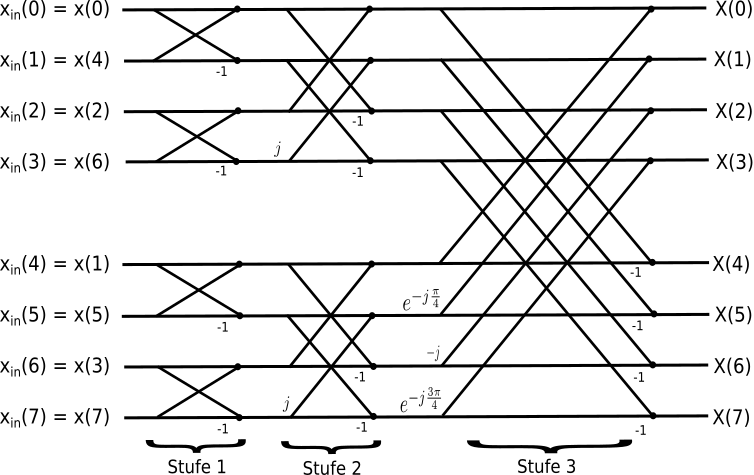
\includegraphics[width=0.7\textwidth]{img/Butterfly.png}
 \caption{Berechnungsschema der DFT mit 8 Eingangswerten nach dem Butterfly-Verfahren}
 \label{pic:Butterfly}
\end{figure}


\subsection{Fazit der Berechnungs-Gegenüberstellungen}
Es konnte gezeigt werden, dass rein von der Anzahl der benötigten Multiplikationen die optimierte Matrixmultiplikation mit komplexen Eingangswerten weniger Multiplikationen
als die FFT hat. Das liegt daran, dass es vom Betrag her nur einen einzigen Faktor gibt. Dieser tritt in vier Zeilen der Twiddlefaktormatrix auf und kann für alle Spalten
der Eingangswerte ausgeklammert werden. Wegen der Spiegelung der Faktoren müssen bei reellen Eingangswerten nur die Hälfte der Multiplikationen durchgeführt werden.
Als Vorteil kann bei der Multiplikation mit komplexen Eingangswerten gesehen werden, dass die Programmierung der 2D-DFT als einfacher angenommen werden kann.
Begründet wird dies damit, dass es möglich ist, die selbe Einheit für die Berechnung der 1D-DFT einfach auch für die 2D-DFT verwenden zu können.
